\subsection{Volume Control Magic: Enhancing HF Reception!}

\begin{tcolorbox}[colback=gray!10, colframe=black, title=E4C11]
     Why does input attenuation reduce receiver overload on the lower frequency HF bands with little or no impact on signal-to-noise ratio?
\begin{enumerate}[label=\Alph*),noitemsep]
    \item The attenuator has a low-pass filter to increase the strength of lower frequency signals
    \item The attenuator has a noise filter to suppress interference
    \item Signals are attenuated separately from the noise
    \item \textbf{Atmospheric noise is generally greater than internally generated noise even after attenuation}
\end{enumerate} \end{tcolorbox}

\subsubsection{Concepts Required to Answer the Question}

To understand why input attenuation affects receiver overload on HF bands while minimally impacting the signal-to-noise ratio (SNR), we must first grasp some fundamental concepts in radio communication:

1. \textbf{Input Attenuation}: This refers to the reduction of the strength of a signal before it is processed by the receiver. Attenuators are typically used to prevent strong signals from overwhelming the receiver's circuitry, particularly in lower frequency bands where signal strength can be more variable.

2. \textbf{Receiver Overload}: This occurs when the incoming signal is too strong for the receiver circuitry, leading to distortion or saturation. This is especially prominent in HF bands where atmospheric conditions can create significant variations in signal strength.

3. \textbf{Signal-to-Noise Ratio (SNR)}: SNR is a measure that compares the level of the desired signal to the level of background noise. A higher SNR indicates a clearer signal reception, while a lower SNR suggests that noise is interfering with the signal.

4. \textbf{Atmospheric Noise}: At lower frequencies, atmospheric noise (from thunderstorms, solar activity, etc.) can be a dominant factor affecting SNR. It tends to be higher than the internally generated noise of the receiver.

\subsubsection{Explaining the Correct Answer}

The correct answer to why input attenuation can help reduce receiver overload on lower frequency HF bands is:

\textbf{D: Atmospheric noise is generally greater than internally generated noise even after attenuation.}

When an attenuator is employed, the incoming signal (which may be strong and lead to overload) is reduced. While both the signal and noise levels are attenuated, it's important to note that atmospheric noise, which exists regardless of the signal level, tends to remain significant compared to the internal noise created by the receiver itself. 

Here's a simplified illustration of the relationship:
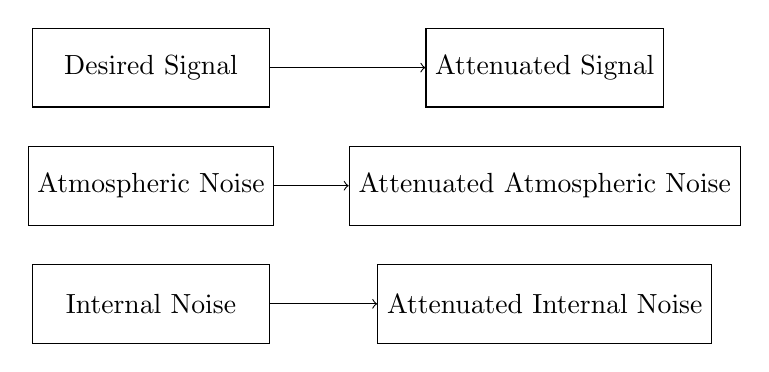
\begin{tikzpicture}
    \node at (0,0) [draw, rectangle, minimum width=3cm, minimum height=1cm] (sig) {Desired Signal};
    \node at (0,-1.5) [draw, rectangle, minimum width=3cm, minimum height=1cm] (atmo) {Atmospheric Noise};
    \node at (0,-3) [draw, rectangle, minimum width=3cm, minimum height=1cm] (int) {Internal Noise};

    \node at (5,0) [draw, rectangle, minimum width=3cm, minimum height=1cm] (atten) {Attenuated Signal};
    \node at (5,-1.5) [draw, rectangle, minimum width=3cm, minimum height=1cm] (atmo2) {Attenuated Atmospheric Noise};
    \node at (5,-3) [draw, rectangle, minimum width=3cm, minimum height=1cm] (int2) {Attenuated Internal Noise};

    \draw[->] (sig.east) -- (atten.west);
    \draw[->] (atmo.east) -- (atmo2.west);
    \draw[->] (int.east) -- (int2.west);
\end{tikzpicture}

Through attenuation, the stronger incoming signal is effectively reduced to prevent overload. However, since the atmospheric noise is relatively larger, its impact remains prominent, and thus the overall SNR is largely unaffected. Consequently, attenuation is beneficial for protecting the receiver without significantly degrading the quality of the received signal. This balance is crucial in keeping the performance of HF receivers optimal in various atmospheric conditions.
